

\tikzset{every picture/.style={line width=0.75pt}} %set default line width to 0.75pt        

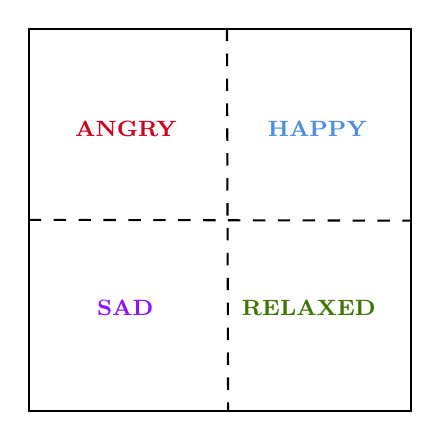
\begin{tikzpicture}[x=0.75pt,y=0.75pt,yscale=-1,xscale=1]
%uncomment if require: \path (0,300); %set diagram left start at 0, and has height of 300


%Shape: Rectangle [id:dp11534307415903555] 
\draw   (148.93,21.48) -- (332.92,21.48) -- (332.92,205.47) -- (148.93,205.47) -- cycle ;
%Straight Lines [id:da7440202322498375] 
\draw  [dash pattern={on 4.5pt off 4.5pt}]  (244.26,21.2) -- (244.82,205.76) ;
%Straight Lines [id:da9738201325291478] 
\draw  [dash pattern={on 4.5pt off 4.5pt}]  (148.75,113.27) -- (332.79,113.69) ;

% Text Node
\draw (169.67,64.48) node [anchor=north west][inner sep=0.75pt]  [font=\footnotesize] [align=left] {\textcolor[rgb]{0.82,0.01,0.11}{\textbf{ANGRY}}};
% Text Node
\draw (262.5,64.48) node [anchor=north west][inner sep=0.75pt]  [font=\footnotesize] [align=left] {\textcolor[rgb]{0.29,0.56,0.89}{\textbf{HAPPY}}};
% Text Node
\draw (180.17,150.48) node [anchor=north west][inner sep=0.75pt]  [font=\footnotesize] [align=left] {\textbf{\textcolor[rgb]{0.56,0.07,1}{SAD}}};
% Text Node
\draw (250,150.48) node [anchor=north west][inner sep=0.75pt]  [font=\footnotesize,color={rgb, 255:red, 65; green, 117; blue, 5 }  ,opacity=1 ] [align=left] {\textbf{RELAXED}};


\end{tikzpicture}
